% Copyright 2021 UChicago Argonne, LLC
% Author:
% - Haoyu Wang and Roberto Ponciroli, Argonne National Laboratory
% - Andrea Alfonsi, Idaho National Laboratory

% Licensed under the Apache License, Version 2.0 (the "License");
% you may not use this file except in compliance with the License.
% You may obtain a copy of the License at

%   https://www.apache.org/licenses/LICENSE-2.0.txt

% Unless required by applicable law or agreed to in writing, software
% distributed under the License is distributed on an "AS IS" BASIS,
% WITHOUT WARRANTIES OR CONDITIONS OF ANY KIND, either express or implied.
% See the License for the specific language governing permissions and
% limitations under the License.

\section{Input of FARM for RAVEN}

In this section, the external matrices file structure, FARM model definition, and input/output file example will be 
discussed. In order to run FARM, two XML files are required:
\begin{itemize}
  \item External Matrices File (See Section \ref{ExtMatFileStructure}), and
  \item Input File (See Section \ref{InputFile})
\end{itemize}
Currently two version of Reference Governor SIMO are provided: paramterized version, and unparameterized version. 
\begin{itemize}
  \item Parameterized Version: Multiple state-space representations profiles are provided in the external matrices file, 
  labeled by a parameter "ActuatorParameter". The FARM will select the closest profile based on the value of input 
  variable "PwrSet".
  \item Unparameterized Version: Single state-space representation profile is provided, and will be used in all the time.
\end{itemize}

\subsection{External Matrices File Structure}
\label{ExtMatFileStructure}
As discussed in \ref{RG_SIMO}, the state space matrices \begin{math} \textbf{A} \end{math}, 
\begin{math} \textbf{B} \end{math}, \begin{math} \textbf{C} \end{math} are required for the FARM to run. 
In addition, the norminal values of 
\begin{math} u \end{math}, 
\begin{math} \overrightarrow{x} \end{math}, 
\begin{math} \overrightarrow{y} \end{math} needs to be known for the following equations at 
\begin{math}k=0 \end{math} to be satisfied:
\begin{itemize}
  \item \begin{math} \overrightarrow{x}[k+1]=\textbf{A}*\overrightarrow{0}+\textbf{B}*0 \end{math}
  \item \begin{math} \overrightarrow{0}=\textbf{C}*\overrightarrow{0} \end{math}
\end{itemize}
In addition, the latest value of \begin{math} \overrightarrow{x} \end{math} needs to be known as the current system state 
if no other values are provided in the Input File.\newline

\subsubsection{Parameterized External Matrices File}
\label{ParaExtMatFile}
The following Listing \ref{lst:ParaExtXMLExample} is a example external matrices file for Parameterized Reference 
Governor with necessary information:

\begin{lstlisting}[style=XML,morekeywords={anAttribute}, 
  caption=Parameterized External Matrices File Example., label=lst:ParaExtXMLExample]
<DataObjectMetadata name="rom_stats">
  <DMDrom type="Static">
    <DMDcModel>
      <dmdTimeScale>1800 1810
      <UNorm>
        <realization ActuatorParameter="-1.15e+01" sample="0">-4.68e-02</realization>
        <realization ActuatorParameter="-3.45e+01" sample="1">-4.30e-01</realization>
      </UNorm>
      <XNorm>
        <realization ActuatorParameter="-1.15e+01" sample="0">2.55e+01 0.00e+00</realization>
        <realization ActuatorParameter="-3.45e+01" sample="1">2.55e+01 0.00e+00</realization>
      </XNorm>  
      <YNorm>
        <realization ActuatorParameter="-1.15e+01" sample="0">3.20e+01 2.55e+01</realization>
        <realization ActuatorParameter="-3.45e+01" sample="1">3.20e+01 2.55e+01</realization>
      </YNorm>
      <XLast>
        <realization ActuatorParameter="-1.15e+01" sample="0">2.44e+01 4.12e+01</realization>
        <realization ActuatorParameter="-3.45e+01" sample="1">2.19e+01 1.38e+02</realization>
      </XLast>
      <Atilde>
        <realization ActuatorParameter="-1.15e+01" sample="0">
          <imaginary>0.00e+00 0.00e+00 0.00e+00 0.00e+00</imaginary>
          <matrixShape>2,2</matrixShape>
          <real>1.00e+00 -1.18e-01 -6.25e-05 4.14e-03</real>
        </realization>
        <realization ActuatorParameter="-3.45e+01" sample="1">
          <imaginary>0.00e+00 0.00e+00 0.00e+00 0.00e+00</imaginary>
          <matrixShape>2,2</matrixShape>
          <real>1.00e+00 -5.61e-02 -6.90e-05 1.32e-01</real>
        </realization>
      </Atilde>
      <Btilde>
        <realization ActuatorParameter="-1.15e+01" sample="0">
          <imaginary>0.00e+00 0.00e+00</imaginary>
          <matrixShape>2,1</matrixShape>
          <real>-2.01e-04 -4.21e+00</real>
        </realization>
        <realization ActuatorParameter="-3.45e+01" sample="1">
          <imaginary>0.00e+00 0.00e+00</imaginary>
          <matrixShape>2,1</matrixShape>
          <real>-2.31e-04 -3.71e+00</real>
        </realization>
      </Btilde>
      <Ctilde>
        <realization ActuatorParameter="-1.15e+01" sample="0">
          <imaginary>0.00e+00 0.00e+00 0.00e+00 0.00e+00</imaginary>
          <matrixShape>2,2</matrixShape>
          <real>-1.00e+00 1.00e+00 -3.48e-10 1.10e-16</real>
        </realization>
        <realization ActuatorParameter="-3.45e+01" sample="1">
          <imaginary>0.00e+00 0.00e+00 0.00e+00 0.00e+00</imaginary>
          <matrixShape>2,2</matrixShape>
          <real>-1.00e+00 1.00e+00 -5.85e-10 7.81e-18</real>
        </realization>
      </Ctilde>
    </DMDcModel>
  </DMDrom> 
</DataObjectMetadata>
\end{lstlisting}

As one can see, all the required information for FARM are included in the \xmlNode{DMDcModel} block. 
Indeed, the name of this block and its parent blocks is flexible:
\begin{itemize}
  \item \xmlNode{DataObjectMetadata}, Root element of XML file, other names are acceptable.
  \item \xmlNode{DMDrom}, Child 1 level element of XML file, other names are acceptable.
  \item \xmlNode{DMDcModel}, Child 2 level element of XML file, other names are acceptable.
\end{itemize}

As long as the following keywords and inputs are the Child 3 level elements of this XML file, the information can 
be processed for FARM execution:
\begin{itemize}
  \item \xmlNode{dmdTimeScale}, \xmlDesc{float vector, required parameter}, 
  the time step marks used in DMDc calculation. 
  At least two consecutive time step value are required to calculate the discrete time interval;
\end{itemize}

Some items (\xmlNode{UNorm}, \xmlNode{XNorm}, \xmlNode{YNorm}, \xmlNode{XLast}, \xmlNode{Atilde}, \xmlNode{Btilde}, 
\xmlNode{Ctilde}) contains multiple \xmlNode{realization} nodes, in the format of 
\xmlNode{realization ActuatorParameter="some float value" sample="some integer value"}, and the corresponding 
values are indexed by this ActuatorParameter. 
\begin{itemize}
  \item 
  \begin{itemize}
    \item The \xmlNode{ActuatorParameter} attribute share the same unit with the input variable "PwrSet", and the 
    parameterized Reference Governor SIMO will select the realization whose \xmlNode{ActuatorParameter} value is 
    closest to the input variable "PwrSet";
    \item The \xmlNode{sample} attribute contains a consecutive integer value starting from 0.
  \end{itemize}
\end{itemize}
All the following items should share the same list of \xmlNode{ActuatorParameter} attribute:
\begin{itemize}
  \item \xmlNode{UNorm}, \xmlDesc{float scalar, required parameter}, 
  the norminal value of system actuation variable \begin{math} u \end{math};
  \item \xmlNode{XNorm}, \xmlDesc{float vector, required parameter}, 
  the norminal value of system state vector \begin{math} \overrightarrow{x}\in\mathbb{R}^n \end{math};
  \item \xmlNode{YNorm}, \xmlDesc{float vector, required parameter}, 
  the norminal value of system output vector \begin{math} \overrightarrow{y}\in\mathbb{R}^p \end{math};
  \begin{itemize}
    \item Note: the \xmlNode{YNorm} must have at least realization that is within the range defined by 
    "Min\_Target" and "Max\_Target" in the definition of Reference Governor SIMO EnternalModel. 
    See Listing \ref{lst:Para_RGSIMOExample} in Section \ref{ParaInputFile}.
  \end{itemize}
  \item \xmlNode{XLast}, \xmlDesc{float vector, required parameter}, 
  the latest value of system state vector \begin{math} \overrightarrow{x}\in\mathbb{R}^n \end{math}, 
  \textbf{without norminal value subtraction};

  \item \xmlNode{Atilde}, \xmlDesc{complex matrix, required parameter}, 
  the state matrix \begin{math} \textbf{A}\in\mathbb{C}^{n \times n} \end{math}:
  \begin{itemize}
    \item \xmlNode{imaginary}, \xmlDesc{float matrix, optional parameter}, 
    the imaginary part of state matrix \begin{math} \textbf{A} \end{math}. The matrix are flattened 
    column-by-column, i.e. the order is 

    \begin{math} A_{11} A_{21} ... A_{n1} \end{math} \begin{math}A_{12} A_{22} ... A_{n2} ... \end{math}
    \item \xmlNode{matrixShape}, \xmlDesc{int vector, required parameter}, 
    the shape of matrix, defined as \xmlNode{matrixShape}Number of Rows,Number of Columns\xmlNode{/matrixShape}
    \item \xmlNode{real}, \xmlDesc{float matrix, required parameter}, 
    the real part of state matrix \begin{math} \textbf{A} \end{math}. The matrix are flattened 
    column-by-column, i.e. the order is 

    \begin{math} A_{11} A_{21} ... A_{n1} \end{math} \begin{math}A_{12} A_{22} ... A_{n2} ... \end{math}
  \end{itemize}
  
  \item \xmlNode{Btilde}, \xmlDesc{complex matrix, required parameter}, 
  the input matrix \begin{math} \textbf{B}\in\mathbb{C}^{n \times 1} \end{math}:
  \begin{itemize}
    \item \xmlNode{real}, \xmlDesc{float matrix, required parameter}, 
    the real part of input matrix \begin{math} \textbf{B} \end{math}. The matrix are flattened 
    column-by-column, i.e. the order is 

    \begin{math} B_{11} B_{21} ... B_{n1} \end{math} \begin{math}B_{12} B_{22} ... B_{n2} ... \end{math}
    \item \xmlNode{matrixShape}, \xmlDesc{int vector, required parameter}, 
    the shape of matrix, defined as \xmlNode{matrixShape}Number of Rows,Number of Columns\xmlNode{/matrixShape}
    \item \xmlNode{imaginary}, \xmlDesc{float matrix, optional parameter}, 
    the imaginary part of input matrix \begin{math} \textbf{B} \end{math}. The matrix are flattened 
    column-by-column, i.e. the order is 

    \begin{math} B_{11} B_{21} ... B_{n1} \end{math} \begin{math}B_{12} B_{22} ... B_{n2} ... \end{math}
  \end{itemize}
  
  \item \xmlNode{Ctilde}, \xmlDesc{complex matrix, required parameter}, 
  the output matrix \begin{math} \textbf{C}\in\mathbb{C}^{p \times n} \end{math}:
  \begin{itemize}
    \item \xmlNode{real}, \xmlDesc{float matrix, required parameter}, 
    the real part of output matrix \begin{math} \textbf{C} \end{math}. The matrix are flattened 
    column-by-column, i.e. the order is 

    \begin{math} C_{11} C_{21} ... C_{n1} \end{math} \begin{math}C_{12} C_{22} ... C_{n2} ... \end{math}
    \item \xmlNode{matrixShape}, \xmlDesc{int vector, required parameter}, 
    the shape of matrix, defined as \xmlNode{matrixShape}Number of Rows,Number of Columns\xmlNode{/matrixShape}
    \item \xmlNode{imaginary}, \xmlDesc{float matrix, optional parameter}, 
    the imaginary part of output matrix \begin{math} \textbf{C} \end{math}. The matrix are flattened 
    column-by-column, i.e. the order is 

    \begin{math} C_{11} C_{21} ... C_{n1} \end{math} \begin{math}C_{12} C_{22} ... C_{n2} ... \end{math}
  \end{itemize}
    
\end{itemize}

This external matrices file example can be found in the following directory, which is automatically generated by a 
Dynamic Mode Decomposition with Control (DMDC)(\cite{proctor2016dynamic} and \cite{wang2020DMDc}) post processor, 
and contains some information that is not necessary for FARM:
\begin{itemize}
  \item /raven/plugins/FARM/tests/RefGov\_para\_xmlABC\_Test/DMDcCxCoeff\_TES\_para.xml
\end{itemize}

This external matrices file represents a thermal energy storage (TES) model, with:
\begin{itemize}
  \item One(1) system actuation variable \begin{math} u \end{math}
  \begin{itemize}
    \item Power set point, measured in Mega Watts (MW);
  \end{itemize}
  \item Two(2)-element system state vector \begin{math} \overrightarrow{x}\in\mathbb{R}^2 \end{math}
  \item Two(2)-element system output vector \begin{math} \overrightarrow{y}\in\mathbb{R}^2 \end{math}
  \begin{itemize}
    \item \begin{math} y_1 \end{math}, Hot fluid tank height, measured in Meter (m);
    \item \begin{math} y_2 \end{math}, Cold fluid tank height, measured in Meter (m);
  \end{itemize}
\end{itemize}

In addition, the state-space representations are parameterized by 20 charging(-)/discharging(+) power levels, 
and the values in \xmlNode{ActuatorParameter} attribute are measured in Mega Watts (MW).

\subsubsection{Unparameterized External Matrices File}
\label{UnparaExtMatFile}
The following Listing \ref{lst:UnparaExtXMLExample} is a example external matrices file for Unparameterized Reference 
Governor with necessary information:

\begin{lstlisting}[style=XML,morekeywords={anAttribute}, 
  caption=Unparameterized External Matrices File Example., label=lst:UnparaExtXMLExample]
<DataObjectMetadata name="rom_stats">
  <DMDrom type="Static">
    <DMDcModel>
      <dmdTimeScale>1800 1810
      <UNorm>
        <realization sample="0">-3.50e+00</realization>
      </UNorm>
      <XNorm>
        <realization sample="0">2.55e+01 0.00e+00</realization>
      </XNorm>
      <XLast>
        <realization sample="0">2.09e+00 9.15e+02</realization>
      </XLast>
      <YNorm>
        <realization sample="0">3.20e+01 2.55e+01</realization>
      </YNorm>
      <Atilde>
        <realization sample="0">
          <imaginary>0.00e+00 0.00e+00 0.00e+00 0.00e+00</imaginary>
          <matrixShape>2,2</matrixShape>
          <real>1.00e+00 -1.33e-02 -5.56e-05 -4.57e-01</real>
        </realization>
      </Atilde>
      <Btilde>
        <realization sample="0">
          <imaginary>0.00e+00 0.00e+00</imaginary>
          <matrixShape>2,1</matrixShape>
          <real>-1.75e-04 -6.25e+00</real>
        </realization>
      </Btilde>
      <Ctilde>
        <realization sample="0">
          <imaginary>0.00e+00 0.00e+00 0.00e+00 0.00e+00</imaginary>
          <matrixShape>2,2</matrixShape>
          <real>-1.00e+00 1.00e+00 -3.76e-11 -4.86e-17</real>
        </realization>
      </Ctilde>
    </DMDcModel>
  </DMDrom>
</DataObjectMetadata>
\end{lstlisting}

As one can see, all the required information for FARM are included in the \xmlNode{DMDcModel} block. 
Indeed, the name of this block and its parent blocks is flexible:
\begin{itemize}
  \item \xmlNode{DataObjectMetadata}, Root element of XML file, other names are acceptable.
  \item \xmlNode{DMDrom}, Child 1 level element of XML file, other names are acceptable.
  \item \xmlNode{DMDcModel}, Child 2 level element of XML file, other names are acceptable.
\end{itemize}

As long as the following keywords and inputs are the Child 3 level elements of this XML file, the information can 
be processed for FARM execution:
\begin{itemize}
  \item \xmlNode{dmdTimeScale}, \xmlDesc{float vector, required parameter}, 
  the time step marks used in DMDc calculation. 
  At least two consecutive time step value are required to calculate the discrete time interval;
\end{itemize}

Some items (\xmlNode{UNorm}, \xmlNode{XNorm}, \xmlNode{YNorm}, \xmlNode{XLast}, \xmlNode{Atilde}, \xmlNode{Btilde}, 
\xmlNode{Ctilde}) contains one \xmlNode{realization} nodes, in the format of 
\xmlNode{realization sample="0"}, and the corresponding value are contained in the \xmlNode{realization} node. 

All the following items have the \xmlNode{realization sample="0"} node:
\begin{itemize}
  \item \xmlNode{UNorm}, \xmlDesc{float scalar, required parameter}, 
  the norminal value of system actuation variable \begin{math} u \end{math};
  \item \xmlNode{XNorm}, \xmlDesc{float vector, required parameter}, 
  the norminal value of system state vector \begin{math} \overrightarrow{x}\in\mathbb{R}^n \end{math};
  \item \xmlNode{YNorm}, \xmlDesc{float vector, required parameter}, 
  the norminal value of system output vector \begin{math} \overrightarrow{y}\in\mathbb{R}^p \end{math};
  \begin{itemize}
    \item Note: the \xmlNode{YNorm} values must be within the range defined by "Min\_Target" and "Max\_Target" in the 
    definition of Reference Governor SIMO EnternalModel. See Listing \ref{lst:Unpara_RGSIMOExample} in Section 
    \ref{UnParaInputFile}.
  \end{itemize}
  \item \xmlNode{XLast}, \xmlDesc{float vector, required parameter}, 
  the latest value of system state vector \begin{math} \overrightarrow{x}\in\mathbb{R}^n \end{math}, 
  \textbf{without norminal value subtraction};

  \item \xmlNode{Atilde}, \xmlDesc{complex matrix, required parameter}, 
  the state matrix \begin{math} \textbf{A}\in\mathbb{C}^{n \times n} \end{math}:
  \begin{itemize}
    \item \xmlNode{imaginary}, \xmlDesc{float matrix, optional parameter}, 
    the imaginary part of state matrix \begin{math} \textbf{A} \end{math}. The matrix are flattened 
    column-by-column, i.e. the order is 

    \begin{math} A_{11} A_{21} ... A_{n1} \end{math} \begin{math}A_{12} A_{22} ... A_{n2} ... \end{math}
    \item \xmlNode{matrixShape}, \xmlDesc{int vector, required parameter}, 
    the shape of matrix, defined as \xmlNode{matrixShape}Number of Rows,Number of Columns\xmlNode{/matrixShape}
    \item \xmlNode{real}, \xmlDesc{float matrix, required parameter}, 
    the real part of state matrix \begin{math} \textbf{A} \end{math}. The matrix are flattened 
    column-by-column, i.e. the order is 

    \begin{math} A_{11} A_{21} ... A_{n1} \end{math} \begin{math}A_{12} A_{22} ... A_{n2} ... \end{math}
  \end{itemize}
  
  \item \xmlNode{Btilde}, \xmlDesc{complex matrix, required parameter}, 
  the input matrix \begin{math} \textbf{B}\in\mathbb{C}^{n \times 1} \end{math}:
  \begin{itemize}
    \item \xmlNode{real}, \xmlDesc{float matrix, required parameter}, 
    the real part of input matrix \begin{math} \textbf{B} \end{math}. The matrix are flattened 
    column-by-column, i.e. the order is 

    \begin{math} B_{11} B_{21} ... B_{n1} \end{math} \begin{math}B_{12} B_{22} ... B_{n2} ... \end{math}
    \item \xmlNode{matrixShape}, \xmlDesc{int vector, required parameter}, 
    the shape of matrix, defined as \xmlNode{matrixShape}Number of Rows,Number of Columns\xmlNode{/matrixShape}
    \item \xmlNode{imaginary}, \xmlDesc{float matrix, optional parameter}, 
    the imaginary part of input matrix \begin{math} \textbf{B} \end{math}. The matrix are flattened 
    column-by-column, i.e. the order is 

    \begin{math} B_{11} B_{21} ... B_{n1} \end{math} \begin{math}B_{12} B_{22} ... B_{n2} ... \end{math}
  \end{itemize}
  
  \item \xmlNode{Ctilde}, \xmlDesc{complex matrix, required parameter}, 
  the output matrix \begin{math} \textbf{C}\in\mathbb{C}^{p \times n} \end{math}:
  \begin{itemize}
    \item \xmlNode{real}, \xmlDesc{float matrix, required parameter}, 
    the real part of output matrix \begin{math} \textbf{C} \end{math}. The matrix are flattened 
    column-by-column, i.e. the order is 

    \begin{math} C_{11} C_{21} ... C_{n1} \end{math} \begin{math}C_{12} C_{22} ... C_{n2} ... \end{math}
    \item \xmlNode{matrixShape}, \xmlDesc{int vector, required parameter}, 
    the shape of matrix, defined as \xmlNode{matrixShape}Number of Rows,Number of Columns\xmlNode{/matrixShape}
    \item \xmlNode{imaginary}, \xmlDesc{float matrix, optional parameter}, 
    the imaginary part of output matrix \begin{math} \textbf{C} \end{math}. The matrix are flattened 
    column-by-column, i.e. the order is 

    \begin{math} C_{11} C_{21} ... C_{n1} \end{math} \begin{math}C_{12} C_{22} ... C_{n2} ... \end{math}
  \end{itemize}
    
\end{itemize}

This external matrices file example can be found in the following directory, which is automatically generated by a 
Dynamic Mode Decomposition with Control (DMDC)(\cite{proctor2016dynamic} and \cite{wang2020DMDc}) post processor, 
and contains some information that is not necessary for FARM:
\begin{itemize}
  \item /raven/plugins/FARM/tests/RefGov\_unpara\_xmlABC\_Test/DMDcCxCoeff\_TES\_unpara.xml
\end{itemize}

This external matrices file represents a thermal energy storage (TES) model, with:
\begin{itemize}
  \item One(1) system actuation variable \begin{math} u \end{math}
  \begin{itemize}
    \item Charging(-)/Discharging(+) Power setpoint, measured in Mega Watts (MW);
  \end{itemize}
  \item Two(2)-element system state vector \begin{math} \overrightarrow{x}\in\mathbb{R}^2 \end{math}
  \item Two(2)-element system output vector \begin{math} \overrightarrow{y}\in\mathbb{R}^2 \end{math}
  \begin{itemize}
    \item \begin{math} y_1 \end{math}, Hot fluid tank height, measured in Meter (m);
    \item \begin{math} y_2 \end{math}, Cold fluid tank height, measured in Meter (m);
  \end{itemize}
\end{itemize}

The state-space representation listed in this external matrices file is linearized at a charging power of 218.5 MW.

\subsection{Input of Reference Governor SIMO ExternalModel}
\label{InputFile}
The input of Reference Governor SIMO is an XML file. 

\subsubsection{Input File for Parameterized Reference Governor SIMO ExternalModel}
\label{ParaInputFile}
An example of the input structure is given in Listing \ref{lst:Para_RGSIMOExample}.
The following section will discuss the different keywords in the input and describe how they are used in this FARM plugin.

\begin{lstlisting}[style=XML,morekeywords={anAttribute},
caption=Reference Governor SIMO ExternalModel Example., label=lst:Para_RGSIMOExample]
  <ExternalModel name="RG1" subType="FARM.RefGov_parameterized_SIMO">
    <outputVariables>V, V_min, V_max</outputVariables>
    <variables>PwrSet, V, V_min, V_max</variables>
    <constant varName="MOASsteps"> 360 </constant>
    <constant varName="Min_Target1"> 2.5 </constant>
    <constant varName="Max_Target1"> 55. </constant>
    <constant varName="Min_Target2"> 2.5 </constant>
    <constant varName="Max_Target2"> 55. </constant>
    <constant varName="Sys_State_x"> 30., 0 </constant>
  </ExternalModel>
\end{lstlisting}

As one can see, all the specifications of the Reference Governor SIMO plugin are given in the \xmlNode{ExternalModel} 
block. 
\begin{itemize}
  \item The \xmlNode{subType} attribute should be set as "FARM.RefGov\_parameterized\_SIMO" to call the parameterized 
  Reference Governor SIMO external model.
\end{itemize}

Inside the \xmlNode{ExternalModel} block, the XML nodes that belong to this plugin only (and not to the ExternalModel) 
are:
\begin{itemize}
  \item \xmlNode{outputVariables}, \xmlDesc{3-element string, required parameter}, the names of output variables:
  \begin{itemize}
    \item Adjusted actuation variable \begin{math} u \end{math}, 
    any user-defined name is allowed(e.g. V);
    \item Lower limit of adjusted actuation variable \begin{math} u \end{math}, 
    any user-defined name is allowed (e.g. V\_min);
    \item Upper limit of adjusted actuation variable \begin{math} u \end{math}, 
    any user-defined name is allowed (e.g. V\_max);
  \end{itemize}
  The order of the 3 variables should be strictly followed.
  
  \item \xmlNode{variables}, \xmlDesc{4-element string, required parameter}, the names of: 
  \begin{itemize}
    \item Original actuation variable \begin{math} r \end{math}, 
    any user-defined name is allowed (e.g. PwrSet);
    \item The 3 output variables in \xmlNode{outputVariables}
  \end{itemize}
  The order of the 4 variables should be strictly followed.
  
  \item \xmlNode{constant varName="MOASsteps"}, \xmlDesc{integer, required parameter},  
  the $\textbf{g}$ value of steps to predict in the future (e.g. 360);
  
  \item And 2*p blocks of \xmlNode{constant} regarding the constraints on system output vector 
  \begin{math} \overrightarrow{y}\in\mathbb{R}^p \end{math}
  \begin{itemize}
    \item \xmlNode{constant varName="Min\_Target1"}, \xmlDesc{float, required parameter}, 
    the lower constraint on output \begin{math} y_1 \end{math} (e.g. 2.5);
    \item \xmlNode{constant varName="Max\_Target1"}, \xmlDesc{float, required parameter}, 
    the upper constraint on output \begin{math} y_1 \end{math} (e.g. 50.);
    \item \xmlNode{constant varName="Min\_Target2"}, \xmlDesc{float, required parameter}, 
    the lower constraint on output \begin{math} y_2 \end{math} (e.g. 2.5);
    \item \xmlNode{constant varName="Max\_Target2"}, \xmlDesc{float, required parameter}, 
    the upper constraint on output \begin{math} y_2 \end{math} (e.g. 50.);
    \item ...
    \item \xmlNode{constant varName="Min\_Targetp"}, \xmlDesc{float, required parameter}, 
    the lower constraint on output \begin{math} y_p \end{math} (not shown in Listing 
    \ref{lst:Para_RGSIMOExample} due to $p=2$);
    \item \xmlNode{constant varName="Max\_Targetp"}, \xmlDesc{float, required parameter}, 
    the upper constraint on output \begin{math} y_p \end{math} (not shown in Listing 
    \ref{lst:Para_RGSIMOExample} due to $p=2$);
  \end{itemize}
  \item \xmlNode{constant varName="Sys\_State\_x"}, \xmlDesc{float vector, optional parameter},
  the current system state vector \begin{math} x \end{math} (e.g. 30., 0) before subtracting 
  the value in \xmlNode{XNorm} in the External Matrice File (See Section \ref{ParaExtMatFile}). 
  If not supplied, the FARM will automatically use the the value in \xmlNode{XLast} in the 
  External Matrice File (See Section \ref{ParaExtMatFile}).
\end{itemize}
This external model definition example can be found in the following directory:
\begin{itemize}
  \item /raven/plugins/FARM/tests/test\_RefGov\_para\_xmlABC.xml
\end{itemize}

and it is designed for a thermal energy storage (TES) simulation, with:
\begin{itemize}
  \item One(1) input variable:
  \begin{itemize}
    \item PwrSet, Charging(-)/Discharging(+) Power setpoint, measured in Mega Watts (MW);
  \end{itemize}
  \item Three(3) output variables:
  \begin{itemize}
    \item V, Adjusted Charging(-)/Discharging(+) Power setpoint, measured in Mega Watts (MW);
    \item V\_min, Admissible power setpoint lower limit, measured in Mega Watts (MW);
    \item V\_max, Admissible power setpoint upper limit, measured in Mega Watts (MW);
  \end{itemize}
  \item MOASsteps \begin{math} g=360 \end{math}, will project for the next 360 discrete time steps;
  \item Two(2) pairs of system output constraints:
  \begin{itemize}
    \item \begin{math} y_1 \end{math}, Hot fluid tank height, measured in Meter (m);
    \item \begin{math} y_2 \end{math}, Cold fluid tank height, measured in Meter (m);
  \end{itemize}
\end{itemize}

\subsubsection{Input File for Unparameterized Reference Governor SIMO ExternalModel}
\label{UnparaInputFile}
An example of the input structure is given in Listing \ref{lst:Unpara_RGSIMOExample}.
The following section will discuss the different keywords in the input and describe how they are used in this FARM plugin.

\begin{lstlisting}[style=XML,morekeywords={anAttribute},
caption=Reference Governor SIMO ExternalModel Example., label=lst:Unpara_RGSIMOExample]
  <ExternalModel name="RG1" subType="FARM.RefGov_unparameterized_SIMO">
    <outputVariables>V, V_min, V_max</outputVariables>
    <variables>PwrSet, V, V_min, V_max</variables>
    <constant varName="MOASsteps"> 360 </constant>
    <constant varName="Min_Target1"> 2.5 </constant>
    <constant varName="Max_Target1"> 55. </constant>
    <constant varName="Min_Target2"> 2.5 </constant>
    <constant varName="Max_Target2"> 55. </constant>
    <constant varName="Sys_State_x"> 30., 0 </constant>
  </ExternalModel>
\end{lstlisting}

Being similar to Listing \ref{lst:Para_RGSIMOExample}, all the specifications of the Reference Governor SIMO plugin 
are given in the \xmlNode{ExternalModel} block. The only difference is 
\begin{itemize}
  \item The \xmlNode{subType} attribute should be set as "FARM.RefGov\_unparameterized\_SIMO" to call the unparameterized 
  Reference Governor SIMO external model.
\end{itemize}

This external model definition example can be found in the following directory:
\begin{itemize}
  \item /raven/plugins/FARM/tests/test\_RefGov\_unpara\_xmlABC.xml
\end{itemize}

and it is designed for the same thermal energy storage (TES) simulation described in Section \ref{ParaInputFile}.

\subsection{Input File Example with FARM.RefGov\_parameterized\_SIMO ExternalModel}

A complete input file example using the external model "FARM.RefGov\_parameterized\_SIMO" can be found in the 
following directory, and it will be discussed in this section:
\begin{itemize}
  \item /raven/plugins/FARM/tests/test\_RefGov\_para\_xmlABC.xml
\end{itemize}
This RAVEN input file simulates the feedback from RefGov\_parameterized\_SIMO ExternalModel. The key factors are:
\begin{itemize}
  \item External matrices file in Listing \ref{lst:ParaExtXMLExample} is used;
  \item External model defined in Listing \ref{lst:Para_RGSIMOExample} is used;
  \item Twenty(20) random input values (uniformly distributed over range [-2000, +2000] MegaWatts) will be generated, 
  and fed into the external model as "PwrSet";
  \item The external model will perform the calculation, and print the three(3) outputs(V, V\_min, V\_max) associated 
  with each input value of PwrSet to a file "RefGovOutput.csv".
\end{itemize}
The example input file is shown in Listing \ref{lst:InputRGSIMOExample}:

\begin{lstlisting}[style=XML,morekeywords={anAttribute},
caption=Input File Example using RefGov.RefGov\_SIMO ExternalModel., label=lst:InputRGSIMOExample]
<Simulation verbosity="silent">
  <TestInfo>
    <name>plugins/FARM.RefGov_parameterized_SIMO</name>
    <author>HaoyuWang</author>
    <created>2021-02-01</created>
    <classesTested>Models.ExternalModel</classesTested>
    <description>
      This is a test run of parameterized reference governor. It loads ABC matrices from external xml file and calculate the feedback from RefGov_parameterized_SIMO external model.
    </description>
    <requirements> </requirements>
  </TestInfo>
  <!-- TestInfo is the description part of input xml file, won't run -->
  
  <RunInfo>
    <WorkingDir>RefGov_para_xmlABC_Test</WorkingDir>
    <Sequence>
      RGrun,
      printTOfile
    </Sequence>
  </RunInfo>
 
  <Files>
    <Input name="ABCMatrices" type="">DMDcCxCoeff_TES_para.xml</Input>
  </Files>

  <Models>
    <ExternalModel name="RG1" subType="FARM.RefGov_parameterized_SIMO">
      <!-- 3 output variables -->  
      <outputVariables>V, V_min, V_max </outputVariables>
      <!-- 4 variables: Issued Setpoint(PwrSet), Adjusted Setpoint(V1), bounds of V1(V1min & V1max) -->
      <variables> PwrSet, V, V_min, V_max </variables>
      <!-- steps in MOAS calculation, "g" value -->
      <constant varName="MOASsteps"> 360 </constant>
      <!-- lower and upper bounds for y vector, will be internally checked -->
      <constant varName="Min_Target1"> 2.5 </constant> 
      <constant varName="Max_Target1"> 55. </constant> 
      <constant varName="Min_Target2"> 2.5 </constant> 
      <constant varName="Max_Target2"> 55. </constant> 
      <!-- System state vector "x", optional, with elements separated by comma(,) -->
      <constant varName="Sys_State_x"> 30.,0 </constant>     
    </ExternalModel>
  </Models>
 
  <Distributions>
    <Uniform name="one">
      <lowerBound>-2000</lowerBound>
      <upperBound>2000</upperBound>
    </Uniform>
  <!-- distribution for PwrSet sampling -->
  </Distributions>

  <Samplers>
    <MonteCarlo name="RG_Sampler">
      <samplerInit>
        <limit>20</limit>
      </samplerInit>
      <variable name="PwrSet">
        <distribution>one</distribution>
      </variable>
    </MonteCarlo>
  <!-- A MonteCarlo sampler for PwrSet sampling  -->
  </Samplers>

  <DataObjects>
    <PointSet name="RGInput">
      <Input>PwrSet </Input>
      <Output>OutputPlaceHolder</Output>
    </PointSet>
    <PointSet name="RGOutput">
      <Input>PwrSet </Input>
      <Output>V, V_min, V_max </Output>
    </PointSet>
  <!-- input and output pointsets for RG -->
  </DataObjects>

  <Steps>
    <MultiRun name="RGrun">
      <Input  class="DataObjects" type="PointSet">RGInput</Input>
      <Input  class="Files" type="">ABCMatrices</Input>
      <Model  class="Models"  type="ExternalModel">RG1</Model>
      <Sampler  class="Samplers"  type="MonteCarlo">RG_Sampler</Sampler>
      <Output class="DataObjects" type="PointSet">RGOutput</Output>
    </MultiRun>
    <!-- MultiRun step to execute the plugin for multiple times -->	
    <IOStep name="printTOfile">
      <Input  class="DataObjects" type="PointSet">RGOutput</Input>
      <Output class="OutStreams"  type="Print">RefGovOutput</Output>
  </IOStep>
  <!-- IOStep to dump the RGOutput to RefGovOutput.csv-->
  </Steps>

  <OutStreams>
    <Print name="RefGovOutput">
      <type>csv</type>
      <source>RGOutput</source>
      <what>input,output</what>
    </Print>
  </OutStreams>
</Simulation>
\end{lstlisting}
The output is a csv file, containing 10 rows of input-outputs (PwrSet - V - V\_min - V\_max). The data and plot are included 
in Figure \ref{fig:RGSIMOoutput}. 

As one can see, the V\_min and V\_max placed limits on the adjusted actuation variable V:
\begin{itemize}
  \item when original actuation variable(PwrSet) exceeds the upper limit(V\_max), the actuation variable(V) is adjusted to 
  V\_max;
  \item when original actuation variable(PwrSet) undergoes the lower limit(V\_min), the actuation variable(V) is adjusted to 
  V\_min;
  \item when original actuation variable(PwrSet) is within the range of [V\_min, V\_max], the actuation variable V has the 
  same value as PwrSet.
\end{itemize}


\begin{figure}[h]
  \centerline{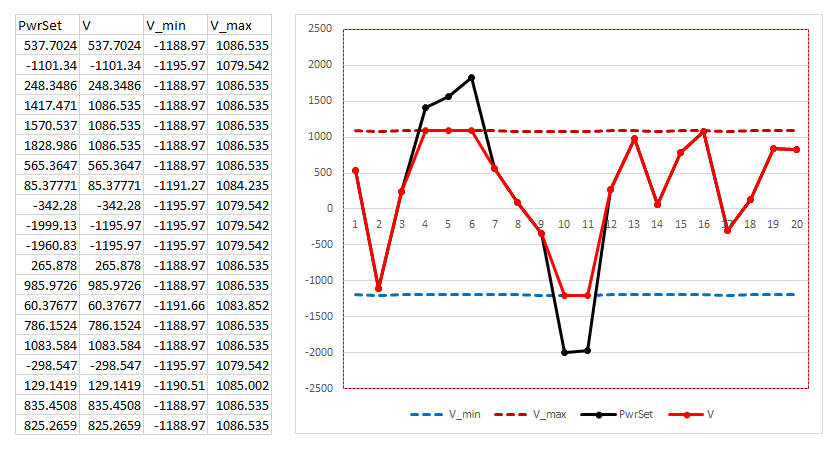
\includegraphics[width=6in]{include/RefGovOutput.png}}
  \caption{Data and Plot from example RefGov\_parameterized\_SIMO input file.}
  \label{fig:RGSIMOoutput}
\end{figure}

